\section{Setup and Preparation}
    \subsection{Working Environment}
    The automatic pet feeder is designed to work on a flat surface (preferably the floor) where your pets will be able to easily access the bowls. Whilst the robot has been designed for stability, we recommend that you place the pet feeder on an even surface to prevent it from being knocked over. To ensure that your pets adjust to their new feeding environment as easily as possible, we advise that you set the pet feeder up in a similar location to where your pets are currently fed. 
    
    \subsection{Network Setup}
    FE.ED requires an internet connection in order to function. Both the raspberry pi and EV3 should automatically connect to the network once they are powered on. This \href{https://cdn-learn.adafruit.com/downloads/pdf/adafruits-raspberry-pi-lesson-3-network-setup.pdf}{guide} provides useful advice on connecting the raspberry pi to a network. For further EV3 information, please refer to section 2.3.1. Alternatively, you can contact our customer support at \href{mailto:support@feed.co.uk}{support@feed.co.uk}.
    
    \subsection{Robot Setup}
    First ensure the pet feeder is set up by placing the robot in a suitable environment as outlined in section 2.1. Make sure the Raspberry Pi is plugged in to the mains supply and the camera view is unobstructed. 

    \subsubsection{EV3 Setup}
    Whilst the EV3 can operate on battery, the charge duration is not sufficient to ensure that the EV3 will be powered when the robot is scheduled to dispense. We advise that the EV3 is plugged in to the mains supply using the 10V/700ma cable provided. To do this connect the charger to the mains, and locate the charging port on the base of the EV3. The green LED indicates a good connection.
    
    \begin{wrapfigure}{r}{0.25\textwidth}
        \centering
        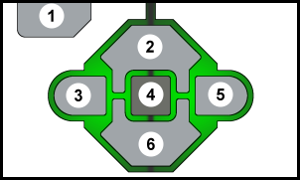
\includegraphics[width=0.25\textwidth]{buttons.png}
         \caption{EV3 Buttons}
    \end{wrapfigure}
 
    
    To power on the EV3 Brick, press and hold the Center (4) button. The Brick Status Light will then turn red and the starting screen will be displayed. When the light changes to green, your EV3 Brick is ready. To turn off the EV3 Brick, press the Back (1) button until you see the Shut Down screen. 
    
    For further information on using the EV3, please see this \href{https://le-www-live-s.legocdn.com/sc/media/files/user-guides/ev3/ev3_user_guide_engb-f24950e6482a3c16e56af0fd72a756fe.pdf}{guide}.
    
    \subsection{Web Application}
    The web application stack is already hosted in the cloud. This means there is no need to install anything to run the web app. Simply open up your favourite browser and go to \url{https://r2feedu.xyz}. Further information on Web App usage is outlined under section 3. 




    
        